\documentclass[]{book}
\usepackage{amsmath,amssymb}
\usepackage{amsthm}
\usepackage{xpatch}
\xpatchcmd\swappedhead{~}{.~}{}{}

\usepackage[T1]{fontenc}
\usepackage[utf8]{inputenc}

\usepackage{parskip}
\usepackage{lmodern}
\usepackage{verbatim}
\usepackage{enumerate}
\usepackage{longtable}
\usepackage{booktabs}


\usepackage{xcolor}
%sudo apt-get install texlive-pictures
\usepackage[all]{xy}

\usepackage{hyperref}

\usepackage[ marginparwidth=3cm, marginparsep=0cm]{geometry}
\usepackage{graphicx}
\usepackage[spanish]{babel}


% Scale images if necessary, so that they will not overflow the page
% margins by default, and it is still possible to overwrite the defaults
% using explicit options in \includegraphics[width, height, ...]{}
\setkeys{Gin}{width=\maxwidth,height=\maxheight,keepaspectratio}
% Set default figure placement to htbp
\makeatletter
\def\fps@figure{htbp}
\makeatother


\providecommand{\tightlist}{%
  \setlength{\itemsep}{0pt}\setlength{\parskip}{0pt}}

  
%remove section numbers
%\setcounter{secnumdepth}{0}

\title{Variables aleatorias discretas}
\author{Hugo J. Bello}
\date{}


\renewcommand{\familydefault}{\sfdefault}
\setcounter{chapter}{3}


\theoremstyle{plain}
\swapnumbers % Switch number/label style
\newtheorem{theorem}{Theorem}[section]
\newtheorem{corollary}[theorem]{Corollary}
\newtheorem{lemma}[theorem]{Lemma}
\newtheorem{claim}{Claim}[theorem]
\newtheorem{axiom}[theorem]{Axiom}
\newtheorem{conjecture}[theorem]{Conjecture}
\newtheorem{fact}[theorem]{Fact}
\newtheorem{hypothesis}[theorem]{Hypothesis}
\newtheorem{assumption}[theorem]{Assumption}
\newtheorem{proposition}[theorem]{Proposition}
\newtheorem{property}[theorem]{Propiedad}
\newtheorem{properties}[theorem]{Propiedades}
\newtheorem{criterion}[theorem]{Criterion}
\theoremstyle{definition}
\newtheorem{definition}[theorem]{Definición}
\newtheorem{note}[theorem]{Nota}
\newtheorem{definitions}[theorem]{Definiciones}
\newtheorem{example}[theorem]{Ejemplo}
\newtheorem{remark}[theorem]{Remark}
\newtheorem{problem}[theorem]{Problem}
\newtheorem{principle}[theorem]{Principle}
\newtheorem{method}[theorem]{Método}
\newtheorem{exercise}[theorem]{Ejercicio}

% for specifying a name
\theoremstyle{definition} % just in case the style had changed
\newcommand{\thistheoremname}{}
\newtheorem{genericthm}[theorem]{\thistheoremname}
\newenvironment{customdef}[1]
  {\renewcommand{\thistheoremname}{#1}%
   \begin{genericthm}}
  {\end{genericthm}}


\begin{document}


\chapter{Variables aleatorias discretas}


\section{Variables aleatorias discretas, definición y
propiedades}

\begin{customdef}{Definición intuitiva de variable aleatoria}
  
Una \textbf{variable aleatoria} es esencialmente un número aleatorio.
Como idea de la definición consideremos un ejemplo. Una moneda es
lanzada tres veces. Todas las posibilidades de este experimento de caras
(\emph{c}) y cruces (\emph{x}) es la siguiente:

\[\Omega = \{ccc, ccx, cxx, cxc, xcc, xxc, xcx, xxx\}\]

Ejemplos de variables aleatorias presentes en este experimento son:

\begin{itemize}
\tightlist
\item
  Número total de caras
\item
  Número de caras menos el de cruces
\item
  Número de tiradas donde aparecen tanto caras como cruces.
\item
  Número de tiradas donde solo aparecen caras
\end{itemize}

Cada uno de estos ejemplos son en el fondo una funciones
(\emph{asociaciones}) de elementos de \(\Omega\) a números reales. Por
ejemplo en la variable aleatoria \emph{número total de caras}

\begin{align*}
\text{Elemento del espacio Muestral} & \longmapsto & \text{Valor de la variable}\\
ccc & \longmapsto & 3\\
ccx & \longmapsto & 2\\
cxx & \longmapsto & 1\\
    & \ldots &0
\end{align*}

Es decir que podemos entender una variable aleatoria como una función

\[ \Omega \to \mathbb{R}\]

Puesto que los valores del experiemento aleatorio presentes en
\(\Omega\) son \textbf{aleatorios} los números reales resultados de la
asociación serán también \textbf{aleatorios}

Nos referiremos a esta asociación como \(X\), el valor \(X=1\) se
referirá pues a las tiradas en las que el número de caras es \(1\).

Una \textbf{variable de aleatoria discreta} es aquella que tomas
solamente un conjunto discreto de valores (número finito o contable de
valores)

En nuestro ejemplo anterior, la variable \(X\) que hemos definido solo
toma los valores \(0\), \(1\), \(2\) y \(3\), así que es discreta.

Si la moneda que hemos considerado en el experimento no está trucada,
cada posibilidad de \(\Omega\) tiene probabilidad \(1/8\) lo que nos
permite conocer la probabilidad de cada valor de \(X\):

\[P(X = 0) = \frac{1}{8}\] \[P(X = 1) = \frac{3}{8}\]
\[P(X = 2) = \frac{3}{8}\] \[P(X = 3) = \frac{1}{8}\]
\end{customdef}

\begin{customdef}{Función de masa de probabilidad}
  
En general, conocer las probabilidades de cada suceso de \(\Omega\)
determina las probabilidades de de los distintos valores de \(X\), a
valor de \(X=x\) denotaremos su probabilidad como

\[p(x) = P(X=x)\]

y puesto que la probabilidad de \(\Omega\) es \(1\), sabemos que si
\(\{x_i\}\) son todos los valores posibles de \(X\),

\[\sum_{i} p(x_i) = P(\Omega) = 1\]

A esta función \(p\) se le denomina función de \textbf{masa de
probabilidad}. Esta función suele denotarse con letras minúsculas, en
ocasiones también mediante la letra \(f\).

En nuestro ejemplo podemos representarla así:

\begin{longtable}[]{@{}l@{}}
\toprule
\endhead
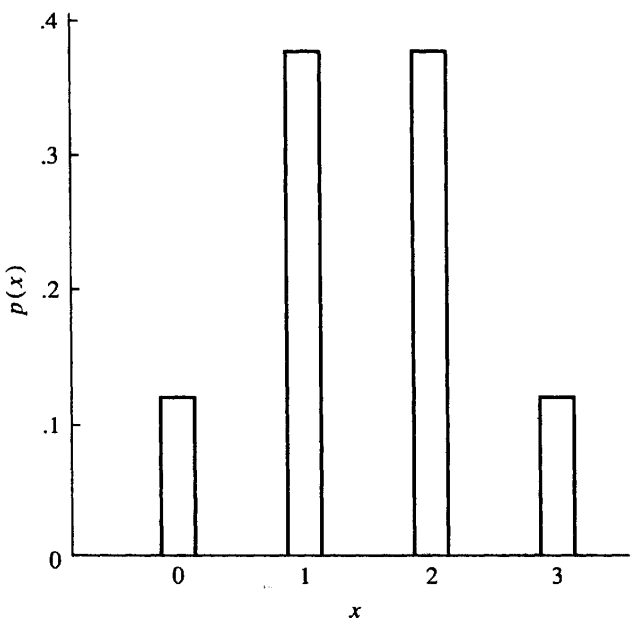
\includegraphics[width=2.60417in,height=\textheight]{img/funcion_masa_discreta.png}\tabularnewline
\bottomrule
\end{longtable}

Además de la función de masa, definimos también la función de
distribución acumulada, de una variable aleatoria como:

\[ F(x) = P(X=x) \text{ para } -\infty < x < \infty\]

Esta función suele denotarse con letras mayusculas.
\end{customdef}

En el ejemplo

\[F(0) = P(X\leq 0) = P(X=0) = \frac{1}{8}\]
\[F(1) = P(X\leq 1) = P(X=0) + P(X=1) = \frac{1}{8} + \frac{3}{8}= \frac{4}{8}\]
\[F(2) = P(X\leq 2) = P(X=0) + P(X=1) + P(X=2) = \frac{1}{8} + \frac{3}{8} + \frac{3}{8} = \frac{7}{8}\]
\[F(3) = P(X\leq 3)  = P(X=0) + P(X=1) + P(X=2) + P(X=3)= \frac{1}{8} + \frac{3}{8} + \frac{3}{8} + \frac{1}{8} =1\]

La siguiente figura representa la función de distribución acumulada del
ejemplo anterior.

\begin{longtable}[]{@{}l@{}}
\toprule
\endhead
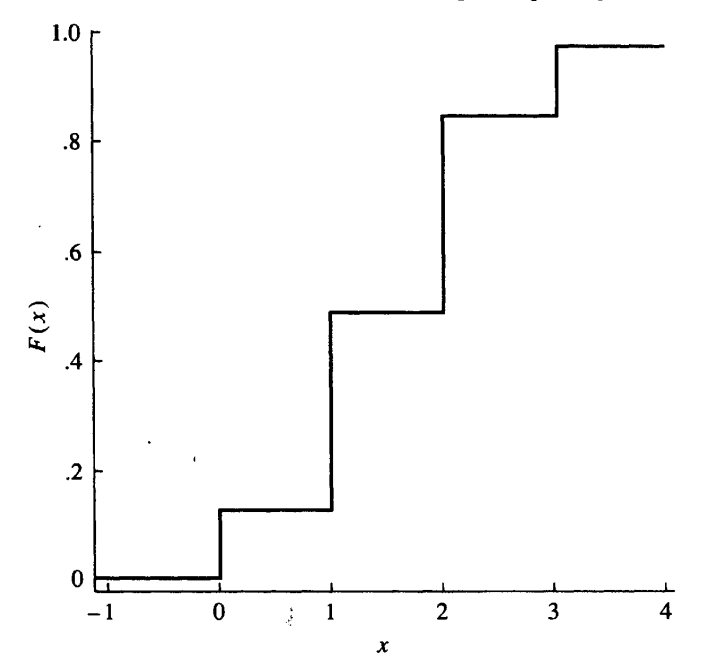
\includegraphics[width=2.60417in,height=\textheight]{img/funcion_dist_acumulada.png}\tabularnewline
\bottomrule
\end{longtable}

Fijemonos que los valores de \(X\) intermedios a los valores
\(0, 1, 2, 3\) el valor de \(F\) es constante, esto se debe a que \(F\)
solo cambia de valor en los valores de \(X\) que corresponden con algún
valor de \(\Omega\).

Observamos que puesto que la probabilidad de \(\Omega\) es \(1\), a
medida que incrementamos los valores de \(X\) en la recta real (eje x de
la gráfica anterior), los valores de \(F(x)\) se acercan más y más a
\(1\), es decir

\[\lim_{x\to\infty} F(x) = 1\]


\section{Esperanza matemática de una variable aleatoria
discreta}

\begin{customdef}{Definición intuitiva de esperanza}
La esperanza matemática (también llamada esperanza, valor
esperado, media poblacional o media) de una variable aleatoria \(X\) ,
es el número \(\displaystyle \mathbb {E} [X]\) que formaliza la idea de
valor medio de un fenómeno aleatorio. Es un concepto análogo a la media
aritmética de un conjunto de datos.

Cuando la variable aleatoria es discreta, la esperanza es igual a la
suma de la probabilidad de cada posible suceso aleatorio multiplicado
por el valor de dicho suceso. Por lo tanto, representa la cantidad
promedio que se \emph{espera} como resultado de un experimento aleatorio
cuando la probabilidad de cada suceso se mantiene constante y el
experimento se repite un elevado número de veces. Cabe decir que el
valor que toma la esperanza matemática en algunos casos puede no ser
esperado en el sentido más general de la palabra (el valor de la
esperanza puede ser improbable o incluso imposible).
\end{customdef}

\begin{definition}
  
Para una variable aleatoria discreta \(X\) con función de distribución
\(p(x)= \displaystyle \operatorname {P} (X=x)\), si denotamos $R_X$ al conjunto de valores que toma $X$,
 la \textbf{esperanza} se define como

\[\displaystyle \operatorname {E} (X)=\sum _{x \in R_x}x\operatorname {P} (X=x) = \sum _{x \in R_x}x\operatorname {p} (x)\]

A menudo a la esperanza $E(X)$ se la denota por la letra griega $\mu$.
\end{definition}

\begin{example}
Por ejemplo, el valor esperado cuando tiramos un dado equilibrado de 6
caras es 3,5. 

Puesto que llamando

\[X=\text{resultado de tirar un dado}\]

En este caso los resultados posibles son $R_X = \{1, 2,3,4,5,6\}$ y podemos hacer el cálculo

\[\displaystyle \begin{aligned}\operatorname {E} (X)=1\cdot {\frac {1}{6}}+2\cdot {\frac {1}{6}}+3\cdot {\frac {1}{6}}+4\cdot {\frac {1}{6}}+5\cdot {\frac {1}{6}}+6\cdot {\frac {1}{6}}\\[6pt]={\frac {1+2+3+4+5+6}{6}}=3.5\end{aligned}\]

y cabe destacar que \(3.5\) no es un valor posible al tirar el dado. En
este caso, en el que todos los sucesos son de igual probabilidad, la
esperanza es igual a la media aritmética.
\end{example}


\begin{example}
  
Una aplicación común de la esperanza matemática es en las apuestas o los
juegos de azar. Por ejemplo, la ruleta francesa tiene 37 casillas
equiprobables. La ganancia para acertar una apuesta a un solo número
paga de 35 a 1 (es decir, cobramos 35 veces lo que hemos apostado). Por
tanto, considerando los 37 posibles resultados, la esperanza matemática
del beneficio para apostar a un solo número es:

\[\displaystyle \left(-1\cdot {\frac {36}{37}}\right)+\left(35\cdot {\frac {1}{37}}\right)\]

que es aproximadamente -0,027027. Por lo tanto uno esperaría, en media,
perder unos 2,7 céntimos por cada euro que apuesta, y el valor esperado
para apostar 1 euro son \(0.972973\) euros. En el mundo de las apuestas,
un juego donde el beneficio esperado es cero (no ganamos ni perdemos) se
llama un \emph{juego justo}.
\end{example}


\begin{property}
  Si $X$ es una variable aleatoria con esperanza finita entonces se cumple que 
  \begin{enumerate}
    \item $E(c) = c$, esto es si $X$ siempre toma el mismo valor $c$ entonces la esperanza coincide con ese valor.
    \item $E[a + b \cdot X] = a + b \cdot E(X)$ para cualesquiera números reales $a,b$.
  \end{enumerate}
  
\end{property}

\section{Varianza de una variable aleatoria
discreta}
\begin{definition}
  Sea \(X\) una variable aleatoria discreta con esperanza
\(\displaystyle \mu =\operatorname {E} (X)\) y función de distribución \(p(x) = \displaystyle \operatorname {P} (X=x)\), se define la varianza de
la variable aleatoria \(X\), denotada por
\(\displaystyle \operatorname {Var} (X)\) como

\[\displaystyle \operatorname {Var} (X)=\operatorname {E} ((X-\mu )^{2}) = \sum _{x\in R_{X}}(x-\mu )^{2}\operatorname {P} (X=x)\]

Donde \(R_X\) denota todos los valores posibles de \(X\).
\end{definition}

\begin{example}
  Si consideramos la variable aleatoria anterior 
  \[X=\text{resultado de tirar un dado}\]
  Vimos que su esperanza era $\mu =  (1+2+3+4+5+6)/6=7/2$, Por lo tanto, la varianza de $X$ es 
  \[
  \begin{aligned}\operatorname {Var} (X)&=\sum _{i=1}^{6}{\frac {1}{6}}\left(i-{\frac {7}{2}}\right)^{2}\\[5pt]&={\frac {1}{6}}\left((-5/2)^{2}+(-3/2)^{2}+(-1/2)^{2}+(1/2)^{2}+(3/2)^{2}+(5/2)^{2}\right)\\[5pt]&={\frac {35}{12}}\approx 2.92.\end{aligned}
  \]
\end{example}

\begin{property}
  Si $X$ es una variable aleatoria con esperanza finita entonces se cumple que 
   \[
    \begin{aligned}\operatorname {Var} (X)&=\operatorname {E} 
      \left[(X-\operatorname {E} [X])^{2}\right]\\[4pt]&=\operatorname {E} 
      \left[X^{2}-2X\operatorname {E} [X]+\operatorname {E} [X]^{2}\right]\\[4pt]
      &=\operatorname {E} \left[X^{2}\right]-2\operatorname {E} [X]\operatorname {E} [X]+
      \operatorname {E} [X]^{2}\\[4pt]&=\operatorname {E} \left[X^{2}\right]-\operatorname {E} [X]^{2}\end{aligned}
 \]
\end{property}

\section{Variables aleatorias de
Bernoulli}

\begin{definition}
  Una \textbf{variable aleatoria de Bernoulli} toma solo dos valores:
\(0\) y \(1\). El valor \(1\) (que representa el éxito en el
experimento) ocurre con la probabilidad \(p\) y el valor \(0\) (que
representa el fracaso en el experimento) con la probabilidad
\(q = 1 - p\).

Cuando una variable \(X\) sigue una distribución de Bernoulli escribimos
\(\displaystyle X\sim \operatorname {Bernoulli} (p)\)

Su función de probabilidad es

\[\displaystyle p(x)=\operatorname {P} (X=x)=p^{x}(1-p)^{1-x}\qquad x=0,1\]

La función de distribución acumulada de una variable aleatoria
\(\displaystyle X\sim \operatorname {Bernoulli} (p)\) está dada por

\[\displaystyle F(x)={\begin{cases}0&x<0\\1-p&0\leq x<1\\1&x\geq 1\end{cases}}\]
\end{definition}

\begin{customdef}{Experimento de Bernoulli}
  Una manera sencilla de entender la variable aleatoria de Bernoulli es pensar que modeliza el experimento más básico que 
  podemos hacer: \emph{Una situación en la que solo pueden darse dos resultados: éxito o fracaso} y la probabilidad de éxito es 
  conocida: $p$. El ejemplo más sencillo de este experimento es justamente tirar una moneda (en este caso la probabilidad de éxito es $1/2$
\end{customdef} 

\begin{property} Si una variable $X$ es  $\operatorname {Bernoulli} (p)$
 \begin{enumerate} [(1)]
   \item $\operatorname {E} \left[X\right]=p$
   \item  $\operatorname {Var} \left[X\right]=p(1-p)$
 \end{enumerate}
  
\end{property}

\begin{proof}
(1) Esta se demuestra fácilmente utilizando la definición de esperanza

\[\displaystyle {\begin{aligned}\operatorname {E} [X]&=0\cdot \operatorname {P} [X=0]+1\cdot \operatorname {P} [X=1]\\&=p\end{aligned}}\]

(2) Con lo anterior es fácil obtener una expresión para
\(\displaystyle \operatorname {E} [X^{2}]\) pues

\[\displaystyle {\begin{aligned}\operatorname {E} [X^{2}]&=\sum _{x=0}^{1}x^{2}p^{x}(1-p)^{1-x}\\&=p(1-p)^{1-1}\\&=p\end{aligned}}\]
 
Teniendo \(\displaystyle \operatorname {E} [X^{2}]\) y
\(\displaystyle \operatorname {E} [X]\) puede deducirse que la varianza
de \(X\) está dada por

\[\displaystyle {\begin{aligned}\operatorname {Var} \left[X\right]&=\operatorname {E} [X^{2}]-\operatorname {E} [X]^{2}\\&=p-p^{2}\\&=p\left(1-p\right)\end{aligned}}\]

\end{proof}

\begin{example}

Tirar una moneda es claramente un ejemplo de variable de Bernoulli. Si
consideramos la correspondencia \(X=0\) como cruz, y \(X=1\) como cara,
\(X\) sigue una variable con una distribución de Bernoulli con
\(p=1/2\), es decir
\(\displaystyle X\sim \operatorname {Bernoulli} (1/2)\)
\end{example}


\section{Distribución Binomial} 

\begin{definition}
  
Supongamos que hacemos \(n\) experimentos independientes o ensayos,
donde \(n\) es un número fijado. Supongamos además que la probabilidad
de \emph{éxito} es \(p\) y la de \emph{fracaso} es \(1-p\).

El número total (después de los \(n\) experimentos) de éxitos, \(X\) es
precisamente una \textbf{variable aleatoria Binomial} con parámetros
\(n\) y \(p\). En este caso escribiremos
\(\displaystyle X\sim \operatorname {Bin} (n,p)\).

Si \(\displaystyle X\sim \operatorname {Bin} (n,p)\) entonces su función
de probabilidad está dada por

\[p(x)=\displaystyle \operatorname {P} (X=x)={n \choose x}p^{x}(1-p)^{n-x}\]

para \(\displaystyle x=0,1,2,\dots ,n\), siendo
\[\displaystyle \!{n \choose x}={\frac {n!}{x!(n-x)!}}\,\!\]

La idea de esto es que \(p^x\) es la probabilidad de haya \(x\) éxitos,
mientras que \((1-p)^{n-x}\) se corresponde con que el resto de intentos
sean fracasos. La razón por la que en la fórmula multiplicamos por
\(n \choose x\) es porque hay exactamente \(n \choose x\) maneras (o
combinaciones) en que pueden aparecer esta proporción de éxitos y
fracasos.

La función de distribución acumulada de una variable aleatoria
\(\displaystyle X\sim \operatorname {Bin} (n,p)\) está dada por

\[\displaystyle F(x)=\operatorname {P} (X\leq x)=\sum _{k=0}^{x}{n \choose k}p^{k}(1-p)^{n-k}\]
\end{definition}

\begin{figure}
  \centering
  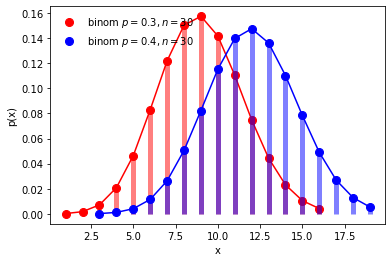
\includegraphics[width=3in,height=\textheight]{img/binom.png}
  \caption{Función de distribución de la variable binomial para varios valores de sus parámetros}
\end{figure}


\begin{property}
  
Si \(\displaystyle X\sim \operatorname {Bin} (n,p)\), entonces 
\begin{enumerate}[(1)]
  \item $\operatorname {E} (X)=np$
  \item $\operatorname {Var} (X)=np(1-p)$
\end{enumerate}
\end{property}


\begin{proof}
  
(1) se deduce del hecho de que la esperanza matemática es lineal y de
que \(X\) es la suma de \(n\) variables aleatorias de Bernoulli

En otras palabras, si\\
\(\displaystyle X_{1},\ldots ,X_{n}\) son identicas e independientes
variables aleatorias Bernoulli con parámetro \(p,\) entonces
\(\displaystyle X=X_{1}+\cdots +X_{n}\) y

\[\displaystyle \operatorname {E} (X)=\operatorname {E} (X_{1}+\cdots +X_{n})=\operatorname {E} (X_{1})+\cdots +\operatorname {E} (X_{n})=p+\cdots +p=np.\]

\end{proof}
 
(2) Para calcular la varianza de una variable binomial, razonamos como en el
apartado anterior:

\[\displaystyle \operatorname {Var} (X)=np(1-p).\]
 



\begin{example}
  
Supongamos que se lanza 51 veces un dado de 6 caras y queremos calcular
la probabilidad de que el número 3 salga 20 veces.

En este problema un ensayo consiste en lanzar el dado una vez.
Consideramos un éxito si obtenemos un 3 pero si no sale 3 lo
consideramos como un fracaso. Defínase \(X\) como el número de veces que
se obtiene un 3 en 51 lanzamientos.

En este caso tenemos
\(\displaystyle X\sim \operatorname {Bin} (51,1/6)\) por lo que la
probabilidad buscada es \(\displaystyle \operatorname {P} (X=20)\)

\[\displaystyle \operatorname {P} (X=20)={51 \choose 20}(1/6)^{20}(1-1/6)^{51-20}=0.0000744\,\!\]

\end{example}
 
\section{Distribución Geométrica} 

\begin{definition}
  
La \textbf{distribución geométrica} se construye también haciendo
múltiples de Bernuoulli con probabilidad de \emph{éxito} es \(p\). La
diferencia respecto a la binomial es que \(X\) será el \emph{número de
experimentos hasta dar con el primer éxito}.

Es decir que \(X=k\) representa \(k-1\) fracasos y \(1\) éxitos. Por lo
tanto

la función de probabilidad de
\(\displaystyle X\sim \operatorname {Geometrica} (p)\) es

\[p(x) = \displaystyle \operatorname {P} (X=x)=p(1-p)^{x-1}\]

para (x=0,1,2,3,\dots )\\

Si \(X\sim \operatorname {Geometrica} (p)\) entonces la función de
distribución acumulada está dada por

\[\begin{aligned}\operatorname {P} (X\leq x)&=\sum _{k=0}^{x}p(1-p)^{k-1}\\&=p\sum _{k=0}^{x}(1-p)^{k-1}\\&=p\left({\frac {1-(1-p)^{x}}{1-(1-p)}}\right)\\&=1-(1-p)^{x}\end{aligned}\]

para (x=0,1,2,3,\dots)
\end{definition}

\begin{figure}
  \centering
  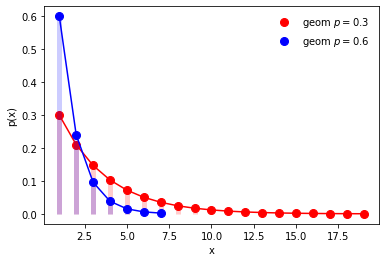
\includegraphics[width=3in,height=\textheight]{img/geom.png}
  \caption{Función de distribución de la variable geométrica para varios valores de sus parámetros}
\end{figure}


\begin{property}
  Si \(X\sim \operatorname {Geometrica} (p)\) entonces
\begin{enumerate}
  \item $\operatorname {E} (X)={\frac {1}{p}}$
  \item $\operatorname {var} (X)={\frac {1-p}{p^{2}}}$
\end{enumerate}
\end{property}


\begin{proof}
  Las demostraciones de estos hechos son un poco más complicada ver:

\begin{itemize}
\tightlist
\item
  \url{https://en.wikipedia.org/wiki/Geometric_distribution}
\end{itemize}
\end{proof}


\begin{example}
   
Se está testando un antidepresivo. La droga puede funcionar o no, pero
hay que testarla en múltiples dosis para ver cual de las tomas funciona.
Por ejemplo la droga puede funcionar al primer intento, al segundo
(segunda dosis), tercero\ldots{} En particular funcione en cualquiera de
las dosis es \(p=0.6\).

¿Cuál es la probabilidad de que funcione a la primera? ¿Y a la segunda?

Fijémonos de que en realidad si llamamos \(X\) al número de tomas
(intentos) hasta que la droga funcione,
\(\displaystyle X\sim \operatorname {Geometrica} (0.6)\)


\[\displaystyle \Pr(X=1)=(1-p)^{1-1}\,p\ =0.4^{0}\times 0.6=0.6\]

\[\displaystyle \Pr(X=2)=(1-p)^{2-1}\,p=0.4^{1}\times 0.6\]
\end{example}

\begin{example} 
Calcular el número de hijos que hay tener hasta tener una niña con
probabilidad más de \(1/2\).
\end{example}



 \section{Distribución Binomial
Negativa} 


\begin{definition}
La distribución Binomial negativa, surge como generalización de la
distribución geométrica. Supongamos que realizamos una secuencia
independiente de experimentos de Bernoulli de probabilidad \(p\), hasta
que obtengamos \(r\) éxitos. Denotemos por \(X\) el número de ensayos
necesarios, en este caso \(X\) será una variable aleatoria binomial
negativa y escribiremos \(\displaystyle X\sim \operatorname {BN} (r,p)\)

Veamos cómo será la función de distribución en este caso. Para encontrar
\(P(X=x)\), pensemos que cada secuencia de experimentos en la que se han
obtenido \(r\) éxitos tiene probabilidad \(p^r(1-p)^{x-r}\).
Obligatoriamente, el último intento debe ser éxito, así que los \(r-1\)
sucesos restantes deben ser asignados entre los \(x-1\) intentos
realizados en \({k-1 \choose r-1}\) maneras. De este modo:

\[P(X=x) = {x-1 \choose r-1} p^r (1-p)^{x-r}\]
\end{definition}



\begin{example}

Si la probabilidad de que un niño expuesto a una enfermedad contagiosa
la contraiga es 0.40 ¿Cuál es la probabilidad de que el décimo niño
expuesto a la enfermedad sea el tercero en contraerla?

En este caso, \(X\) es el número de niños expuestos a la enfermedad
hasta encontrar el tercero en contraer la enfermedad.

\(\displaystyle \!x=10,k=3,p=0.40\)

La solución es:
\[\displaystyle {10-1 \choose 3-1}0,\!4^{3}(1-0,4)^{10-3}={9 \choose 2}0,\!4^{3}(0,\,6)^{7}=0,\!0644973\]
\end{example}

\begin{example}

En un proceso de manufactura se sabe que un promedio de 1 en cada 10
productos es defectuoso, ¿cual es la probabilidad que el quinto (5)
artículo examinado sea el segundo (2) en estar defectuoso? La solución
es:

X= número de artículos que deben ser examinados hasta encontrar dos
defectuoso

\[\displaystyle {5-1 \choose 2-1}0,\!1^{2}(1-0,\!1)^{5-2}={4 \choose 0}0,\!1^{2}(0,\,9)^{3}\]
de probabilidad que el quinto elemento extraído sea el primero en estar
defectuoso.
\end{example}

\begin{property}
  Si \(\displaystyle X\sim \operatorname {BN} (r,p)\)
  \begin{enumerate}[(1)]
    \item $E(X) = r/p$
    \item $V(X) = r(1-p)/p^2$
  \end{enumerate}
\end{property}

\begin{proof}
  Para hacernos a una idea de cómo demostrar esto, basta entender que si $X$ es binomial negativa podemos entender $X$ como la suma
  de $r$ variables geométricas independientes $X_i$. 
  En este caso $X_i = $ número de intentos hasta obtener un acierto, es decir $X_i \sim Geom (p)$.


  Teniendo esto en cuenta 

  \[E(X)= E(\sum^r_{i=1} X_i) = r \sum^r_{i=1} E[X_i] = r/p \]
  \[V(X)= V(\sum^r_{i=1} X_i) = r \sum^r_{i=1} V[X_i] = r(1-p)/p \] 

  Para la varianza hemos usado el hecho de que son independientes, si no no podemos afirmar que la varianza de las sumas 
  la suma de las varianzas.
\end{proof}

\section{Distribución Hipergeométrica} 

\begin{definition}
  Supongamos que, a diferencia que en la distribución Binomial, tenemos un
conjunto de \(N\) objetos, que además pertenecen a dos categorías (dos
tipos o clases). La categoría \(A\) contiene a \(K\) de los objetos y la
categoría \(B\) los restantes \(N-K\).

La distribución hipergeomética mide \textbf{la probabilidad de obtener
\(x\) objetos de la categoría \(A\)} después de \(n\) intentos.

\[\displaystyle p(x)=P(X=x)={\frac {{\binom {K}{x}}{\binom {N-K}{n-x}}}{\binom {N}{n}}},\]

donde

\begin{itemize}
\tightlist
\item
  \(N\) es el número total de objetos,
\item
  \(K\) número de objetos en la categoría \(A\), (posibles éxitos),
\item
  \(n\) número de intentos,
\item
  \(x\) número de objetos de la categoría A observados (éxitos)
\end{itemize}

Para entender el porqué de la fórmula anterior, pensemos en que
\({\binom {K}{x}}\) se corresponden con las maneras que podemos extraer
los \(k\) éxitos (objetos en la categoría \(A\)), mientras que
\({\binom {N-K}{n-x}}\) corresponde con las maneras en que podemos
obtener los \(n-x\) fracasos (objetos en la categoría \(B\)). El
producto de estos dos números combinatorios nos da los \emph{casos
favorables}, los \emph{casos posibles} en cambio los obtenemos con
\({\binom {N}{n}}\).

Habitualmente la categoría A se identifica como los \emph{éxitos} y los de la B como fracasos. 
Entendamos que esta terminología de categoría A y B es simplemente para dar nombres a los elementos, y habitualmente omitiremos 
estos nombres.

\end{definition}

\begin{figure}
  \centering
  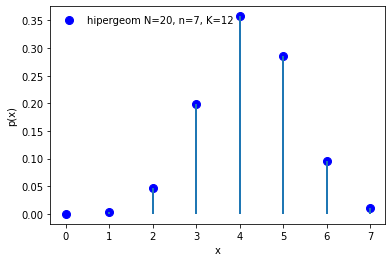
\includegraphics[width=3in,height=\textheight]{img/hipergeom.png}
  \caption{Función de distribución de la variable hipergeométrica}
\end{figure}

\begin{property}

  Si \(\displaystyle X\sim \operatorname {HG} (N,K,n)\)  
\begin{enumerate}
  \item $\displaystyle \operatorname {E} (X)={\frac {nK}{N}}$
  \item $\displaystyle \operatorname {Var} (X)={\frac {nK}{N}}{\bigg (}{\frac {N-K}{N}}{\bigg )}{\bigg (}{\frac {N-n}{N-1}}{\bigg )}$
\end{enumerate}
\end{property}
 
La distribución hipergeométrica es aplicable a muestreos sin reemplazo y
la binomial a muestreos con reemplazo. En situaciones en las que el
número esperado de repeticiones en el muestreo es presumiblemente bajo,
puede aproximarse la primera por la segunda. Esto es así cuando N es
grande y el tamaño relativo de la muestra extraída, n/N, es pequeño.

\begin{example}
Supongamos que hay diez automóviles disponibles para que usted los
pruebe \((N = 10)\) y cinco de ellos tienen motores turbo \((K = 5)\).
Si prueba tres de los vehículos al azar \((n = 3)\), ¿cuál es la
probabilidad de que dos de los tres que pruebe tengan motores turbo?
\end{example}

\begin{example}
 Una empresa fabrica plumas estilográficas. La empresa afirma a sus inversores que tal solo un 1 por ciento de 
 sus plumas son defectuosas. Un perito toma un paquete de 300 y se dispone a testarlas extrayéndolas del paquete, 
 en su peritaje extraerá solamente 5. Suponiendo que 
 lo que afirma la empresa sea cierto
 \begin{enumerate}
   \item ¿Cuántas defectuosas espera encontrar tras sus 5 extracciones?
   \item ¿Cuál es la probabilidad de que encuentre 1 defectuosa tras sus 5 extracciones?
 \end{enumerate}
 
 Para resolver esto, asumimos que es cierto que solo una de cada 100 es defectuosa. Por lo tanto en nuestro paquete hay 300, 
 tendremos que hay 3 defectuosas y 297 no defectuosas. esto es $K=3$, $N=300$, $n=5$.
 \[E(X) = 5 \frac{3}{300} = 0.05\]

 Este valor decimal podemos interpretarlo como espera encontrar 0 plumas defectuosas.

 Para el segundo apartado

 \[p(1) = \frac {{\binom {3}{1}}{\binom {300-3}{5-1}}}{\binom {300}{5}} = \frac{3 \cdot 971435}{19582837560} \cong 0.00014 \]
  
  \end{example}
 
\section{Distribución de Poisson} 

\begin{definition}
  La distribución de Poisson es una distribución de probabilidad discreta
que expresa, a partir de una frecuencia de ocurrencia media, la
probabilidad de que ocurra un determinado número de eventos durante
cierto período de tiempo. Concretamente, se especializa en la
probabilidad de ocurrencia de sucesos con probabilidades muy pequeñas, o
sucesos \emph{raros}.

La distribución de Poisson es popular porque modela el número de veces
que ocurre un evento en un intervalo de tiempo.

Sea \(\displaystyle \lambda >0\) y \(X\) una variable aleatoria
discreta, si la variable aleatoria \(X\) tiene una distribución de
Poisson con parámetro \(\lambda\) entonces escribiremos
\(\displaystyle X\sim \operatorname {Poisson} (\lambda )\)

Si \(\displaystyle X\sim \operatorname {Poisson} (\lambda )\) entonces
la función de probabilidad es

\[\displaystyle \operatorname {P} (X=k)={\frac {e^{-\lambda }\lambda ^{k}}{k!}}\]

donde (k=0,1,2, \dots ) es el número de ocurrencias del evento o
fenómeno.

El parámetro \(\displaystyle \lambda >0\) representa el número de veces
que se espera que ocurra el fenómeno durante un intervalo dado. Por
ejemplo, si el suceso estudiado tiene lugar en promedio 4 veces por
minuto y estamos interesados en la probabilidad de que ocurra k \(k\)
veces dentro de un intervalo de 10 minutos, usaremos un modelo de
distribución de Poisson con \(\lambda = 10\cdot 4 = 40\).
\end{definition}


\begin{figure}
  \centering
  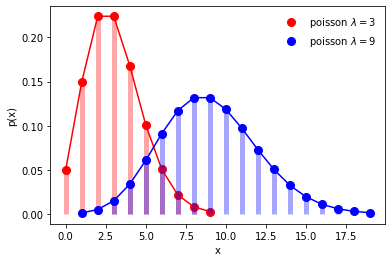
\includegraphics[width=3in,height=\textheight]{img/poisson.png}
  \caption{Función de distribución de la variable Poisson para varios valores de sus parámetros}
\end{figure}

\begin{property}
  
Si \(\displaystyle X\sim \operatorname {Poisson} (\lambda )\) entonces
la variable aleatoria \(X\) satisface  

\begin{enumerate}[(1)]
  \item $\displaystyle \operatorname {E} (X)=\lambda$
  \item $\displaystyle \operatorname {Var} (X)=\lambda $
\end{enumerate}
 
\begin{proof}
  (1) se demuestra por definición de esperanza matemática

\[\displaystyle {\begin{aligned}\operatorname {E} [X]&=\sum _{k=0}^{\infty }k\left({\frac {e^{-\lambda }\lambda ^{k}}{k!}}\right)\\&=e^{-\lambda }\sum _{k=1}^{\infty }{\frac {k\lambda ^{k}}{k!}}\\&=e^{-\lambda }\sum _{k=1}^{\infty }{\frac {\lambda ^{k}}{(k-1)!}}\\&=\lambda e^{-\lambda }\sum _{k=1}^{\infty }{\frac {\lambda ^{k-1}}{(k-1)!}}\\&=\lambda e^{-\lambda }\sum _{j=0}^{\infty }{\frac {\lambda ^{j}}{j!}}\\&=\lambda e^{-\lambda }e^{\lambda }\\&=\lambda \end{aligned}}\]
 
\end{proof}

\end{property}

Es decir, tanto el valor esperado como la varianza de una variable
aleatoria con distribución de Poisson son iguales a \(\lambda\) .


\begin{example}
  
Si el \(\displaystyle 2\%\) de los libros encuadernados en cierto taller
tienen encuadernación defectuosa, para obtener la probabilidad de que 5
de 400 libros encuadernados en este taller tengan encuadernaciones
defectuosas usamos la distribución de Poisson, si se define \(X\) como
el número de libros que tengan encuadernación defectuosa entonces
\(\displaystyle k=5\) y \(\lambda\) (el valor esperado de libros
defectuosos) es el \(\displaystyle 2\%\) de 400 es decir, 8. Por lo
tanto, la probabilidad buscada es:

\[\displaystyle \operatorname {P} (X=5)={\frac {8^{5}e^{-8}}{5!}}=0.092\]
\end{example}

\begin{example}
  El número de soldados muertos por coces de caballos en un año en la caballería Prusiana sigue una distribución de Poisson.
  Este ejemplo fue introducido 
  en un libro por Ladislaus Bortkiewicz (1868--1931) 23-25. 
  Según este autor la media de soldados que mueren por coces de caballos es de
\(\lambda = 0.61\), y se sabe que esta sigue una distribución de
Poisson, calcular la probabilidad de que: 1. Mueran 0 soldados este año
2. Mueran menos de 3
\end{example}

\hypertarget{relaciuxf3n-con-la-binomial}{%
\subsection{Relación con la
binomial}\label{relaciuxf3n-con-la-binomial}}

La distribución de Poisson es el caso límite de la distribución
binomial. De hecho, si los parámetros \(n, p\) de una distribución
binomial tienden a infinito (en el caso de n) y a cero (en el caso de
\(p\) de manera que \(\lambda = np\) se mantenga constante, la
distribución límite obtenida es de Poisson. 

\subsubsection{Procesos de Poisson}

La distribución de Poisson se aplica a varios fenómenos discretos de la
naturaleza (esto es, aquellos fenómenos que ocurren 0, 1, 2, 3,
\ldots{}, veces durante un periodo definido de tiempo o en un área
determinada) cuando la probabilidad de ocurrencia del fenómeno es
constante en el tiempo o el espacio. Ejemplos de estos eventos que
pueden ser modelados por la distribución de Poisson incluyen:

\begin{itemize}
\tightlist
\item
  El número de autos que pasan a través de un cierto punto en una ruta
  (suficientemente distantes de los semáforos) durante un periodo
  definido de tiempo.
\item
  El número de errores de ortografía que uno comete al escribir una
  única página.
\item
  El número de llamadas telefónicas en una central telefónica por
  minuto.
\item
  El número de servidores web accedidos por minuto.
\item
  El número de animales muertos encontrados por unidad de longitud de
  ruta.
\item
  El número de mutaciones de determinada cadena de ADN después de cierta
  cantidad de radiación.
\item
  El número de núcleos atómicos inestables que se han desintegrado en un
  determinado período.
\item
  El número de estrellas en un determinado volumen de espacio.
\item
  La distribución de receptores visuales en la retina del ojo humano.
\item
  La inventiva de un inventor a lo largo de su carrera.
\end{itemize}

\hypertarget{bibliografuxeda}{%
\section{Bibliografía}\label{bibliografuxeda}}

\begin{itemize}
\tightlist
\item
  John A. Rice. Mathematical Statistics and Data Analysis
\item
  F. M. Dekking, C. Kraailkamp, H. P. Lopuhaa, L. E. Meester. A Modern
  Introduction to Probability and Statistics. Understanding Why and How.
\item
  \url{https://es.wikipedia.org/wiki/Distribuci\%C3\%B3n_Bernoulli}
\item
  \url{https://es.wikipedia.org/wiki/Distribuci\%C3\%B3n_binomial}
\item
  \url{https://es.wikipedia.org/wiki/Distribuci\%C3\%B3n_geom\%C3\%A9trica}
\item
  \url{https://es.wikipedia.org/wiki/Distribuci\%C3\%B3n_hipergeom\%C3\%A9trica}
\end{itemize}

\end{document}